%----------
%   WARNING
%----------

% This Guide contains Library recommendations based mainly on APA and IEEE styles, but you must always follow the guidelines of your TFG Tutor and the TFG regulations for your degree.

% THIS TEMPLATE IS BASED ON THE IEEE STYLE 


%----------
% DOCUMENT SETTINGS
%----------

\documentclass[12pt]{report} % font: 12pt

% margins: 2.5 cm top and bottom; 3 cm left and right
\usepackage[
a4paper,
vmargin=2.5cm,
hmargin=3cm
]{geometry}

% Paragraph Spacing and Line Spacing: Narrow (6 pt / 1.15 spacing) or Moderate (6 pt / 1.5 spacing)
\renewcommand{\baselinestretch}{1.15}
\parskip=6pt

% Color settings for cover and code listings 
\usepackage[table]{xcolor}
\definecolor{azulUC3M}{RGB}{0,0,102}
\definecolor{gray97}{gray}{.97}
\definecolor{gray75}{gray}{.75}
\definecolor{gray45}{gray}{.45}

% PDF/A -- Important for its inclusion in e-Archive. PDF/A is the optimal format for preservation and for the generation of metadata: http://uc3m.libguides.com/ld.php?content_id=31389625. 

% In the template we include the file OUTPUT.XMPDATA. You can download that file and include the metadata that will be incorporated into the PDF file when you compile the memoria.tex file. Then upload it back to your project.  
\usepackage[a-1b]{pdfx}

% LINKS
\usepackage{hyperref}
\hypersetup{
    colorlinks=false,      % text color always black
    pdfborder={0 0 1},     % activates rectangle thing(1 = width)
    pdfborderstyle={/S/U}, % (S=solid, D=dashed, U=underline)
    linkbordercolor={1 0 0},  % red
    urlbordercolor={0 0 1},   % blue 
    citebordercolor={0 1 0}   % green
}

% MATH EXPRESSIONS
\usepackage{amsmath,amssymb,amsfonts,amsthm}

% Character encoding
\usepackage[T1]{fontenc}
\usepackage[utf8]{inputenc}

% Times New Roman (text + math)
\usepackage{newtxtext,newtxmath}


% English settings
\usepackage[english]{babel} 
\usepackage[babel, english=american]{csquotes}
\AtBeginEnvironment{quote}{\small}

% Footer settings
\usepackage{fancyhdr}
\pagestyle{fancy}
\fancyhf{}
\renewcommand{\headrulewidth}{0pt}
\rfoot{\thepage}
\fancypagestyle{plain}{\pagestyle{fancy}}

% DESIGN OF THE TITLES of the parts of the work (chapters and epigraphs or sub-chapters)
\usepackage{titlesec}
\usepackage{titletoc}
\titleformat{\chapter}[block]
{\large\bfseries\filcenter}
{\thechapter.}
{5pt}
{\MakeUppercase}
{}
\titlespacing{\chapter}{0pt}{0pt}{*3}
\titlecontents{chapter}
[0pt]                                               
{}
{\contentsmargin{0pt}\thecontentslabel.\enspace\uppercase}
{\contentsmargin{0pt}\uppercase}                        
{\titlerule*[.7pc]{.}\contentspage}                 

\titleformat{\section}
{\bfseries}
{\thesection.}
{5pt}
{}
\titlecontents{section}
[5pt]                                               
{}
{\contentsmargin{0pt}\thecontentslabel.\enspace}
{\contentsmargin{0pt}}
{\titlerule*[.7pc]{.}\contentspage}

\titleformat{\subsection}
{\normalsize\bfseries}
{\thesubsection.}
{5pt}
{}
\titlecontents{subsection}
[10pt]                                               
{}
{\contentsmargin{0pt}                          
	\thecontentslabel.\enspace}
{\contentsmargin{0pt}}                        
{\titlerule*[.7pc]{.}\contentspage}  


% Tables and figures settings
\usepackage{multirow} % combine cells 
\usepackage{caption} % customize the title of tables and figures
\usepackage{floatrow} % we use this package and its \ ttabbox and \ ffigbox macros to align the table and figure names according to the defined style.
\usepackage{array} % with this package we can define in the following line a new type of column for tables: custom width and centered content
\newcolumntype{P}[1]{>{\centering\arraybackslash}p{#1}}
\DeclareCaptionFormat{upper}{#1#2\uppercase{#3}\par}
\usepackage{graphicx}
\graphicspath{{imagenes/}} % Images folder

% Table layout for engineering
\captionsetup*[table]{
	format=plain,
	name=TABLE,
	justification=raggedright,
	labelsep=period,
	width=.75\linewidth,
	labelfont=small,
	font=small
}

% Figures layout for engineering
\captionsetup[figure]{
	format=hang,
	name=Fig.,
	singlelinecheck=off,
	labelsep=period,
	labelfont=small,
	font=small		
}

% FOOTNOTES
\usepackage{chngcntr} % continuous numbering of footnotes
\counterwithout{footnote}{chapter}

% CODE LISTINGS 
% support and styling for listings. More information in  https://es.wikibooks.org/wiki/Manual_de_LaTeX/Listados_de_código/Listados_con_listings
\usepackage{listings}

% Custom listing
\lstdefinestyle{estilo}{ frame=Ltb,
	framerule=0pt,
	aboveskip=0.5cm,
	framextopmargin=3pt,
	framexbottommargin=3pt,
	framexleftmargin=0.4cm,
	framesep=0pt,
	rulesep=.4pt,
	backgroundcolor=\color{gray97},
	rulesepcolor=\color{black},
	%
	basicstyle=\ttfamily\footnotesize,
	keywordstyle=\bfseries,
	stringstyle=\ttfamily,
	showstringspaces = false,
	commentstyle=\color{gray45},     
	%
	numbers=left,
	numbersep=15pt,
	numberstyle=\tiny,
	numberfirstline = false,
	breaklines=true,
	xleftmargin=\parindent
}

\captionsetup*[lstlisting]{font=small, labelsep=period}
 
\lstset{style=estilo}
\renewcommand{\lstlistingname}{\uppercase{Código}}


% REFERENCES 

% IEEE bibliography setup
\usepackage[backend=biber, style=ieee, isbn=false,sortcites, maxbibnames=6, minbibnames=1]{biblatex} % Setting for IEEE citation style, recommended for engineering. "maxbibnames" indicates that from 6 authors truncate the list in the first one (minbibnames) and add "et al." as used in the IEEE style.

\addbibresource{referencias.bib} % The references.bib file in which the bibliography used should be

\usepackage{tikz}
\usetikzlibrary{shapes, arrows, positioning, fit}
\usepackage{subcaption}
\usepackage{booktabs}

\usepackage{xcolor}
\definecolor{myblue}{RGB}{39,123,167}
\setlength{\fboxrule}{1pt}
\setlength{\fboxsep}{0pt}

%-------------
%	DOCUMENT
%-------------

\begin{document}
\pagenumbering{roman} % Roman numerals are used in the numbering of the pages preceding the body of the work.
	
%----------
%	COVER
%----------	
\begin{titlepage}
	\begin{sffamily}
	\color{azulUC3M}
	\begin{center}
		\begin{figure}[H] % UC3M Logo
			\makebox[\textwidth][c]{\includegraphics[width=16cm]{logo_UC3M.png}}
		\end{figure}
		\vspace{2.5cm}
		\begin{Large}
			Bachelor Degree in Computer Science \& Engineering\\			
			 2025-2026\\ % Academic year
			\vspace{2cm}		
			\textsl{Bachelor Thesis}
			\bigskip
			
		\end{Large}
		 	{\Huge  Advancing Plant Phenotyping in Rangelands Through Drone-Derived Imagery and Video Data }\\
		 	\vspace*{0.5cm}
	 		\rule{10.5cm}{0.1mm}\\
			\vspace*{0.9cm}
			{\LARGE Javier Martín Pizarro}\\ 
			\vspace*{1cm}
		\begin{Large}
			Joao Ricardo Pereira Valente\\
			Leganés, Madrid\\
            March, 2026\\
		\end{Large}
	\end{center}
	\vfill
	\color{black}
	% IF OUR WORK IS TO BE PUBLISHED UNDER A CREATIVE COMMONS LICENSE, INCLUDE THESE LINES. IS THE RECOMMENDED OPTION.
	\includegraphics[width=4.2cm]{creativecommons.png}\\ % Creative Commons Logo
    This work is licensed under Creative Commons \textbf{Attribution – Non Commercial – Non Derivatives}
	\end{sffamily}
\end{titlepage}

\newpage % blank page
\thispagestyle{empty}
\mbox{}

%----------
%	ABSTRACT AND KEYWORDS 
%----------	
\renewcommand\abstractname{\large\bfseries\filcenter\uppercase{ABSTRACT}}
\begin{abstract}
\thispagestyle{plain}
\setcounter{page}{3}
	
	% Write your abstract
    Site-specific weed control (SSWC) has been a problem since humans started to develop the field of agriculture. During the ages, existing methodologies did not change at all: they were based on manual detection and extraction. However, this changed with the appearance of modern computers.

    In the last fifty years, there has been an extreme evolution in the detection of non-desired weeds. However, it was not until recently that newer computational methodologies based on Deep Learning and Artificial Neural Networks --- more specifically Convolutional Neural Networks --- were introduced into the field that the advances became trully efective.

    This work addresses the development of a computer vision model capable of locating and counting instances of \textit{Eryngium horridum}---commonly known as "cardilla"—--a perennial, spiny weed species native to the grasslands of Uruguay, Argentina, and southern Brazil. By leveraging drone-derived imagery and video data, this thesis aims to contribute to precision agriculture and ecological monitoring, enhancing the sustainability and efficiency of rangeland management practices.

    \vfill
    
	\textbf{Keywords:} % add the keywords
    Site-specific Weed Control, Object Counting, Object Segmentation, Computer Vision, Artificial Intelligence

    \vspace*{2cm}

\end{abstract}
	\newpage % Blank page
	\thispagestyle{empty}
	\mbox{}


%----------
%	Dedication
%----------	
\chapter*{Dedication}

\setcounter{page}{5}
	
	I would like to dedicate this work to the two fundamental pillars of my life:

    To my family. You have been there for me no matter what. Even when I did not deserve it. You will always be the beacon I need when I must return to safe ports.

    To my brothers. We are not blood-related, but you will always have a seat at my table. With you, I found loyalty even in the worst of the storms.
		
	\vfill

    \begin{flushright}
    \begin{minipage}{0.7\textwidth}
        \textit{" We will all die and the universe will carry on without care.
        All that we have is that shout into the wind—how we live.
        How we go. And how we stand before we fall. "}
    
        \vspace{0.3cm}
        \end{minipage}
        \\
        --- Pierce Brown, \textit{Golden Son}
    \end{flushright}


    \vspace{2cm}
	
	\newpage % blank page
	\thispagestyle{empty}
	\mbox{}
	

%----------
%	TOC
%----------	

%--
% TOC
%-
\tableofcontents
\thispagestyle{fancy}

\newpage % blank page
\thispagestyle{empty}
\mbox{}

%--
% List of figures. If they are not included, comment the following lines
%-
\listoffigures
\thispagestyle{fancy}

\newpage % blank page
\thispagestyle{empty}
\mbox{}

%--
% List of tables. If they are not included, comment the following lines
%-
\listoftables
\thispagestyle{fancy}

\newpage % blankpage
\thispagestyle{empty}
\mbox{}

%----------
%	THESIS
%----------	
\clearpage
\pagenumbering{arabic} % numbering with Arabic numerals for the rest of the document.	

\chapter{Introduction and Motivation}

The purpose of this chapter is to introduce the topic of the thesis, present the current state of the art --- from both theoretical and practical perspectives --- and outline the motivations behind it, as well as the regulatory framework and the associated economic impact.

\section{Motivation}

Agriculture plays a crucial role in the economy of the vast majorities of the countries in the world. Although in developed countries such as Spain it plays a less important role (near 2.3\% in 2024\cite{worldbank2024}), in some developing countries such as Hispanic America it can raise up to 8\%.

\begin{figure}[H]
    \centering
    \includegraphics[width=0.75\linewidth]{imagenes/world_bank_group_pib.jpg}
    \caption{Gross Domestic Product (GDP) share of agriculture, forestry, and fishing (in \%) between the years 1960 and 2024.
    Source: \textit{World Bank Data} \cite{worldbank2024}.}
    \label{fig:worldbank_gdp}
\end{figure}

Maintaining an adequate rhythm of production is vital not only for the economy, but for sustaining the quality of life of the population. Thus, innovating with new technologies in this field has always been necessary to supply the increasing demand.

Weeds have been consistently a problem; not only they reduced the quality and quantity of the crops, but detecting them was an extenuating job. Until the development of modern machinery, it was mainly done by hand --- covering entire fields and removing them --- or using agriculture techniques for avoiding their apparition --- mainly grazing and crops rotation ---, with mediocre results.

In the early years of the XX century, tractors were starting to be more and more common, reducing manual labour activities a lot. However, there was still the possibility of developing weeds in the fields and not being able of estimating the total amount of them in the total land size.

Estimating the amount per hectare (or other desired unit of measure) is vital for understanding how weeds are influencing in the growth and quality of crops. Depending on the density of these unwanted plants, different quantities of herbicides can be used, reducing toxins and improving the condition of the batches.

Modern computation technologies were firstly used near the 70s: archaic solutions based on reflecting-based living ("green") plants with photoelectric diodes\cite{Coleman2022} were proposed. However, these methods were highly dependant on the ability of controlling the constantly in-change environment.

In the 80s, with the appearance of digital cameras, a new bunch of possibilities appeared. As the spectral-colour range cameras were more and more affordable, a totally new world for exploring this field was discovered.

The first predecessor of formal Convolutional Neural Networks --- known as the neocognitron ---, presented by Kunihiko Fukushima was a totally game-changer. It was a multilayer perceptron (MLP) able to extract features and predict handwritten numerals from "0" to "9"\cite{FUKUSHIMA1988119}. Fukushima also proposed several unsupervised training algorithms. Although they were revolutionary, after the proposal of back-propagation \cite{ACKLEY1985147} (which is heavily used in computer vision currently) they fell into disuse.

After it, a spiral of hype and constant changes for these neural networks came into scene. In 1998, the LeNet-5\cite{Lecun98} was the first neural network to include back-propagation end-to-end which was tested with the MNIST dataset.

In 2012, the neural network AlexNet was proposed. With nearly 22,000 categories (labels), this neural network was able to generalise a vast number of different objects with high precision. However, the most innovative thing was that it was \textbf{trained using Graphics Processing Units --- GPUs ---}\cite{Alex2012}, something that was never used in the field. This rapidly raised the level of training methodologies, reducing the time elapsed.

Only three years later, Microsoft engineers proposed a new method to lighten the weight of neural networks. After benchmarking and stating that \textbf{"the deeper network has higher training error, and thus test error"}\cite{Kaiming2015}. This means that the more layers a network has (above a critical limit), the less precise it gets. They propose the Deep Residual Learning, based on the difference (error) between the expected value and the obtained one.

$$F(x) = H(x) - x$$
$$y = F(x) + x$$

Using this approach, the net eases the learning process compared to the standards of the moment. As a subsequent effect, they are able to reduce the weight of the networks up to an 80\% (compared with VGG nets).

It was not until 2012 that convolutional neural networks were mature enough in order to be applied in the agriculture field. However, there are important limitations when using these methodologies --- which are by far the most effective---.

The main limitation is not computational or algorithmic, but the datasets used for training the nets. It is common to have a very limited dataset with very few instances of useful data to preprocess and work with. Restricted to the regions where they were obtained, it is complicated to make a dataset that is representative for an extensive region. 

Nonetheless, the region is not the only factor, but also the seasons of the year. Generating a fine dataset that shows every phenotype of a given plant in a specific moment is expensive --- economically and humanly ---.

Thus, the aim of this work is not only to create a model able to segment and count instances of the cardilla, but to create a dataset competent enough to provide the sufficient information for future works about the field.

\subsection{About the \textit{Eryngium horridum}}
\label{subsec:aboutEryngium}

Original from Hispanic America, the \textit{Eryngium horridum} ---also known as cardilla or caraguatá--- is common to locate in the plain lands of Uruguay, southern Brazil and central-eastern Argentina.

The plant is a perennial forb with a highly distinctive morphology; it is a rosette with numerous spiny linear leaves that can reach up to 65 cm in length and 2 cm in width. Its inflorescence axis can grow as tall as 2 meters \cite{Quinones2025}.

\begin{figure}[H]
    \centering
    \includegraphics[width=0.75\linewidth]{imagenes/eryngium_horridum.jpg}
    \caption{\textit{Eryngium Horridum}: Left image: bottom part of the plant. Upper right: flower. Bottom left: inflorescence}.
    \label{fig:eryngium_horridum}
\end{figure}

One peculiarity of this plant is its resilience in adverse conditions. After experiencing fires or frosts, it has been mentioned to see the floral part of the stem to grow quicker and bigger than before.

Although there are no common uses for this plant, it is known that it helps in the scarring process. However, here ends its applications. It is not harvested, at the contrary, it is heavily prosecuted because of the rapid growing through fields, destroying useful terrain for cropping in a few months. Not even the livestock desires to eat it, unless excessive hunger.

A quickly identification of the plant is needed to solve the issue before it ruins the field and the crops already planted.

\subsection{Technical challenge}

Although it is clearly obvious the distinctive shape of the plant, trying to observe them from an aerial perspective gets much more complicated. Depending on the height of the UAV (Unmanned Aerial Vehicle) and the quality and resolution of the camera, the difficulty can increase exponentially.

\begin{figure}[H]
    \centering
    \includegraphics[width=0.75\linewidth]{imagenes/aerialfield.png}
    \caption{Recorded aerial view from an unknown height. Sizes differ between each individual deppending on different factors, such as the dryness of the plant.}
    \label{fig:aerial_eryngium}
\end{figure}

Estimating the possibles individuals per hectare by hand, even with the help of UAVs, is complex enough. In the last ten years, the trend of computer vision has also arrived to this field.

\textbf{Computer vision}, which a field of artificial intelligence --- more specifically from machine learning ---, is a discipline that allows computers to process images (frames) and to extract meaningfully data and make decisions.

This challenge is based on the Multiple Object Tracking (MOT); which aims for identifying an arbitrary number of $n$ individuals with the maximum precision possible.

In the literature, there are currently two approaches for solving the MOT problem: \textbf{Detection-based Tracking (DBT)} and \textbf{Detection-Free Tracking (DFT)}. Whereas the DBT is used an external and automatic detector for localising the objects in the frame, the DFT needs some manual input at first glance in order to keep up with the trajectory of the item.

\begin{figure}[H]
	\centering
	\includegraphics[width=0.75\linewidth]{imagenes/mot_types.pdf}
	\caption{Visual representation of the MOT problem. The multiplexer determines the approach: either Detection-based Tracking or Detection-Free Tracking.}
	\label{fig:mot_types}
\end{figure}

These approaches, although similar, are not used in the same use cases. The applications differ, as well as the advantages and disadvantages depending on the scenaries where they are used.

\begin{table}[H]
    \centering
        \begin{tabular}{lcc}
        \toprule
        \textbf{Variables} & \textbf{DBT} & \textbf{DFT} \\
        \midrule
        Initialization & automatic, possibly imperfect & manual, perfect \\
        \# of objects & varying & fixed \\
        Applications & specific type of objects & any types of objects \\
        Advantages & ability to handle varying number of objects & free of object detector \\
        Disadvantages & performance depends on object detection & manual initialization \\    
		\bottomrule
    \end{tabular}
    \caption{Comparison between DBT and DFT. Adapted from \cite{LUO2021103448}}
    \label{tab:dbt_vs_dft}
\end{table}

Whereas the DBT is made up from a pipeline: the \textbf{detector} (in charge of predicting the boxes of the items) and the \textbf{asociator} (in charge of asociating each box with a label or class) and then uses associations algorithms (see \ref{subsec:asoc_algorithm}) for identifying the movement of an object, the DFT is much more complex. The net itself learns how to predict the trayectory of the individual, using transformers and tokens for maintining the individual identity of the model.

At first, DFT may seem like a reasonable option to choose. However, its complexity its not trivial. It is important to mention that usually is required to have big datasets for these types of models. In this work, the quantity and quality of the frames are not as large and precise as it would be prefereable. Thus, Detection-Based Tracking is a better option.

\begin{itemize}
	\item Freedom for controlling the detector (YOLO, Faster R-CNN...)
	\item Atomic: is easier to modify local features.
	\item Different methods of association can be used for experimenting with them.
\end{itemize}

In summary, while both DBT and DFT approaches seems to be good enough results, the \textbf{Detection Based Tracking} method can give us more interpretability and control while developing the framework, specially with the data limitations of this study.

Therefore, the main focus of this study will be on the DBT pipeline, combining different classification models with associations algorithms. However, to evaluate the potential of more recent and capable technologies, the \textbf{T-Rex 2} model \cite{Jiang2024trex2} --- a representative of the DFT family --- will be also tested as a comparative benchmark. 

From this technical review, several questions arise:

\begin{enumerate}
	\item How effectively can a detection-based model identify, localize and track the \textit{Eryngium horridum}?
	\item How do supervised models performed (DBT) compared to end-to-end transformers-based arquitectures such as T-Rex 2 (DFT)?
	\item What are the limitations and generalization capabilities of these models when faced across different plant densities, flight altitudes, and observation perspectives?
\end{enumerate}

The source code developed for this project is publicly accessible on GitHub, baptised as CARLA --- Cardilla Recognition and Localization Analyzer \cite{repoGithub}.

\section{State of Art: An introduction to Object Detection and Segmentation}

\subsection{Associations Algorithms}
\label{subsec:asoc_algorithm}

\section{Regulatory Framework}

\subsection{European Regulatory Framework}

The regulatory framework about these emerging technologies --- such as AI and UAVs --- are still being defined worlwide. In the European Union, several laws about the usage of AI and UAVs have been already defined for the correct usage of both technologies. 

\subsubsection{European Regulatory Framework of UAVs}

Unmanned Aerial Vehicles regulatory framework started to develop in the early 2020s, with the approval of the Implementing Regulation (UE) 2019/947, which defines the rules and procedures for the usage of drones in european aerial space and the Implementing Regulation (UE) 2018/1139, which integrated the drone normative with the European Union Aviation safety Agency (EASA).

One of the most important points of this regulation is the classification of the drones: \textit{open}, \textit{specific} or \textit{certified}, which depends on several factors such as the danger of the mission and the capabilities of the vehicle. Depending on the category of the vehicle, different requirements may be needed (for the pilot and the plane) to fly in european space.

\begin{enumerate}
	\item \textbf{Open}: \textit{low danger operations}. Most are recreational or simple comercial flights. No previous authorization is required is the drone follows several requirements: weight does not surpass 25 kg, maximum flight altitude is 125 meters high and the vehicle will not approach any vital infraestructure (such as airports). The pilot must have constantly visual sight of the vehicle.
	\item \textbf{Specific}: \textit{medium danger operations}. In this category, flights required to have a previous authorization of the corresponding authorities (AESA in Spain). However, the limitations of these flights are less restricted than in the open category: night operations, increase size and weight of the vehicle and the posibility of flying in urban zones.
	\item \textbf{Certified}: \textit{high danger operations}. Compared to traditional aviation operations. This category includes vehicles that transports passengers or dangerous commodities or that used autonomous flights without any possible human interaction. Currently, there are very few operations that are currently in the need of this category; it is aimed for future projects.
\end{enumerate}

In addition, the law in Spain (and thus in the entire European Union) requires that every drone pilot must be certified with a license, obtaining an unique identity number valid in the entire European Union.

This work aims to contribute to the open and specific categories. Here, individuals such as farmers or researchers may be in the need of using drones for recognising and identifying weeds in their fields. 

However, these services can be also done through a company specialized in this. The pilots the company must be certified pilots as well. And because of the high amount of flights per week that these pilots may need to do, exists the \textbf{Light UAS Operator Certificate} (LUC) for frequent operators. These operators do not need to ask for previous authorization to AESA, reducing the bureocracy and speeding up the process of asking for authorization, which can last up to ten working days. 

\subsubsection{European Regulatory Framework of Artificial Intelligence}

In 2024 the European Union adopted the first worldwide normative with respect to artificial intelligence: the reglament (UE) 2024/1689, also known as the Law of Artificial Intelligence or AI Act. It is defined as a machine-based system designed to operate between different levels of autonomy. 

The AI Act introduces a well-defined categorization of risk for AI systems. Depending on the risk category, some systems are forbidden, whereas others may require and extensive assessment before market entry.

\begin{itemize}
	
	\item \textbf{Unacceptable risk}: applications such as social scoring systems and manipulative technologies are absolutely banned in the EU. 
	\item \textbf{High risk}: applications based on risk evaluation (such as risk or infraestructure) must pass strict compliance reviews.
	\item \textbf{Limited risk}: limited applications such as recommender systems, image or video processing and more need to clarify to the user its usage and the usage of AI for generating the output. Data quality, transparency and fairness standards are required even for these types of applications  
	\item \textbf{Minimal risk}: spam filters or or AI in video games fall in this category. They are not subjected to any regulatory framework.

\end{itemize}

The work proposed in this document clearly falls into the \textit{limited risk} category. Thus, it is important to remark that transparency and fairness are vital. This is because the output of an AI model could cause confussion or influence decision-making capabilities of the user. 

Several mininmal obligations are required to these systems for the sake of the protection of the user:

\begin{itemize}
	\item User must always know that is using AI.
	\item Artificially generated contents must be labeled as "AI Generated" in order to avoid confusion or wiles.
	\item A transparent design means a less biased model.
	\item It is recommended to include ethics by design. This can be done by evaluating biases during training or applying \textit{algorithmical justice}
\end{itemize}

The AI Act also mentions that the systems must be explainable (XAI). The goal of XAI is quite ambitious: surpassing the black box issue and integrating algorithms with human values, empowering and enhancing the individual in the decision-making process \cite{ALI2023101805}. 


\subsubsection{European Regulatory Framework of Personal Data and Privacy}

In Europe, every use of personal data needs to follow the privacy policy established by the European Union; more specifically the GDPR --- General Data Protection Regulation --- which its effective date was 2018. 

The GDPR imposes some fundamental principles about the usage of data, which can be used in AI proyects. These principles are based on transparency, loyalty and legality. Moreover, a limitation must be setted for the usage of the data in order to prevent a misuse of it.

Furthermore, the data must be stored following the principles of integrity and confidentiality up to an arbitrary number of years defined during the process of collection.

One relevant change that of the GDPR is that the population has rights about its own data: they have the right to access, change, remove or oppose to their usage in some applications. This means that every institution that automates processes using AI must be transparent about their usage and how it arrive to the conclusion given, which again bring us to XAI (eXplainable AI).

It is important to mention that the GDPR and AI Act were created to coexist: if an institution want to apply a service using AI, it must subjected to both the AI Act and the GDPR. 

\subsection{Regulatory Framework in Hispanic America}

In contrast to the European Union’s harmonized legal ecosystem, Hispanoamerica presents a more fragmented regulatory landscape regarding artificial intelligence, data privacy, and UAV (drone) operations. However, several countries have made considerable advances toward regulating these technologies, particularly in the areas of \textbf{data protection} and \textbf{civil aviation}.

\subsubsection{Data Protection and Privacy Laws}

Many Hispanoamerican countries have enacted specific laws to regulate the collection, processing, and use of personal data, largely inspired by international frameworks such as the EU's GDPR. 

\begin{itemize}
    \item \textbf{Brazil} enacted the \textit{Lei Geral de Proteção de Dados} (LGPD - Law No. 13.709/2018), a comprehensive data protection law closely modeled after the GDPR, which applies to both public and private sector data handling. It includes principles such as consent, purpose limitation, data minimization, and accountability, and is enforced by the national authority ANPD.
    
    \item \textbf{Argentina} was a pioneer with its Data Protection Law 25.326, which regulates personal data processing and guarantees data subject rights. The law also prohibits the dissemination of image or video data containing identifiable individuals without prior consent.
    
    \item \textbf{Chile}, \textbf{Mexico}, and \textbf{Uruguay} have similar legislative frameworks, each including provisions that require informed consent, secure data processing, and individuals’ right to access or correct their data. In Uruguay, the Law 18.331 governs personal data protection and is overseen by the Unidad Reguladora y de Control de Datos Personales (URCDP).
\end{itemize}

These national frameworks establish that any AI or drone-based system capturing or processing images, biometrics, or location data must comply with consent and purpose principles. This significantly affects agricultural or surveillance applications involving UAVs or computer vision.

\subsubsection{AI-Specific Legislative Developments}

Unlike the EU’s AI Act, Hispanoamerica does not yet have unified legislation targeting artificial intelligence. Nevertheless, several countries have launched national AI strategies and draft bills focused on ethical guidelines, transparency, and fostering innovation.

\begin{itemize}
    \item \textbf{Brazil} released its \textit{Estratégia Brasileira de IA} (2021), outlining policy objectives including responsible AI, scientific research, and AI in public services. A federal AI Bill was proposed in 2022 and is under parliamentary discussion.
    
    \item \textbf{Chile} introduced its National AI Policy in 2021, emphasizing development based on human rights, inclusion, and explainability.
    
    \item \textbf{Argentina}, \textbf{Colombia}, and \textbf{Uruguay} are also developing their national frameworks, supported by regional cooperation through organizations like CEPAL and the IADB.
\end{itemize}

Though still in progress, these initiatives aim to provide a regulatory basis for ethical AI deployment in agriculture, education, and digital public infrastructure.

\subsubsection{UAV and Drone Legislation}

Drone regulations in Hispanoamerica vary considerably by country. However, civil aviation authorities generally restrict operational parameters such as maximum altitude, speed, and flight over populated areas.

\begin{itemize}
    \item In \textbf{Brazil}, the National Civil Aviation Agency (ANAC) regulates UAVs through RBAC-E94, which establishes over 70 provisions for certification, weight categories, and operation types. Drones used for commercial, agricultural, or research purposes require operator registration, flight authorization, and in some cases, insurance.

    \item \textbf{Argentina} maintains similar strict controls, requiring UAV registration, operator licenses, and compliance with maximum altitude (120 m) and speed (161 km/h) limits \cite{Sanchez23}.

    \item In contrast, \textbf{Uruguay} has a more permissive regime for recreational drones: no formal permit is required for sport or leisure flights, provided that basic safety measures are followed and no sensitive areas are overflown.

    \item Countries such as \textbf{Colombia}, \textbf{Peru}, and \textbf{Mexico} follow hybrid approaches based on international aviation safety standards, including pilot certification and risk assessment for advanced operations (e.g., BVLOS, agricultural spraying).
\end{itemize}

Overall, while regulation is less standardized than in Europe, most Hispanoamerican countries are actively updating their frameworks to address UAV usage, particularly as drone-based AI systems become more prevalent in agriculture, infrastructure monitoring, and environmental surveillance.

\section{Socio-economic impact}

something

\section{Planification and budget}

\clearpage

\chapter{Dataset}

The dataset elaboration is usually the most expensive part of the project (in terms of human labour), specially when working with such a complicated problem. In this chapter, the methodologies for the data collection and the analysis of it are explained in detail, commenting the difficulties found when labelling the images and critically analizing the final result of it.

\section{Data Collection Procedures}
\label{section:dataCollectionProcedures}

The collection of the entire dataset was done in the Treinta y Tres department of Uruguay (-33.253618º S, -54.503245º W in WGS84 (World Geodetic System 1984), 52 m a.s.l.). The team in charge was located at the "Palo a Pique" Research Station from the National Institute of Agricultural Research (in Spanish: Instituto Nacional de Investigación Agropecuaria).


\begin{figure}[H]
    \centering
    \includegraphics[width=0.75\linewidth]{imagenes/dataLocationObtainer.pdf}
    \caption{Dataset collection location. The image was obtained through Google Maps.}
    \label{fig:datasetCollectionLocation}
\end{figure}


For the aerial recording of the environment, the usage of a quadcopter was necessary. The aerial platform was a quadcopter, DJI Mavic Air 2, equipped with an integrated RGB sensor, model FC3170, aperture of f/2.8, exposure time of 1/500 s, and focal distance of 4 mm. The flight was made on 21 October 2024, at noon with a clear sky. The flight was scheduled on a cross-path over 0.4 ha, at 10 m altitude (this can vary depending on the frame), with 75 \% frontal and 70 \% lateral overlap, and a camera angle of 75 ° (this varies in some videos in order to obtain different angles of view from the same point) (adapted from \cite{Quinones2025}).

In order to increase the posibilities of experiments for this works, videos were recorded in two modalities: \textbf{RGB} and \textbf{hyperspectral}. RGB stands for Red, Green and Blue, which combined in different measures different colors can be generated.

\begin{figure}[H]
	\centering
	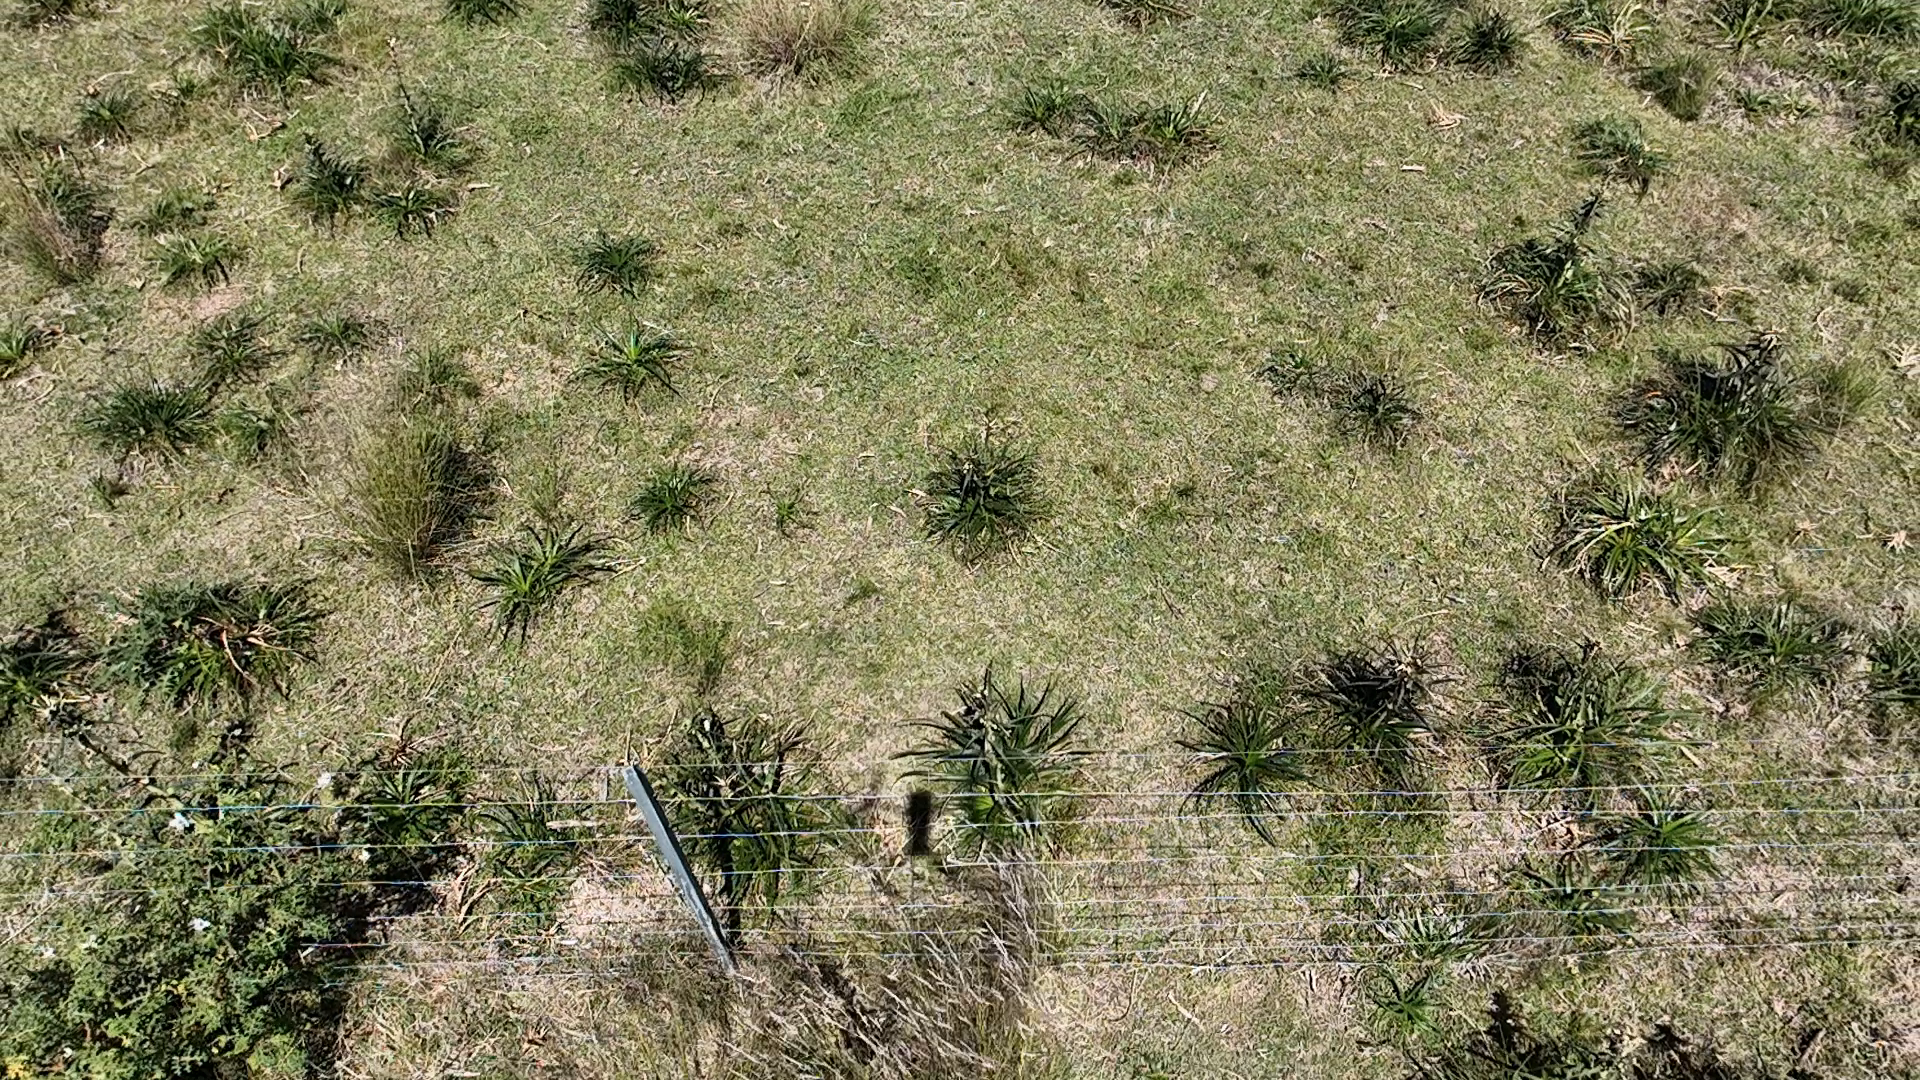
\includegraphics[width=0.75\linewidth]{imagenes/dataset/rgb_frame.png}
	\caption{A frame from the RGB dataset. In this case, weeds can be easily identified due to its size and color constract with respect to the soil.}
	\label{fig:rgbCardilla}
\end{figure}

On the other hand, hyperspectral is based on traditional imaging with a combination of spectroscopy to capture detailed information across a give range of wavelenghts. Spectroscopy is the study of how matter and electromagnetic radiation interact between other through absorption, emission or scattering.

\begin{figure}[H]
	\centering
	\includegraphics[width=0.75\linewidth]{imagenes/dataset/hyperspectral_frame.png}
	\caption{The corresponding hyperspectral image for \ref{fig:rgbCardilla}. Notice they slightly differ between each other.}
	\label{fig:hyperspectralCardilla}
\end{figure}

As it is possible to see in the previous image \ref{fig:hyperspectralCardilla}, the specimens of the weed can be clearly distinguished from the soil and other minor vegetation, adding an extra layer of precision for its detection.

For the same flight, both modes were used. However, due to external factor the videos are not exactly the same so the corresponding frames neither are. A script was executed to reduce these differences to the minimum.

The entire dataset frame collection has lasted, at least, one year --- as it started on the October 22, 2024 and at the current date of writing this document (December 1, 2025) more data is currently being recorded for increasing the size of the dataset.

\section{Data Analysis}

This part embraces the entirety of a defined pipeline in order to incorporate the frames obtained from the videos into the dataset. The following diagram represents the pipeline used:

\begin{figure}[H]
    \centering
    \includegraphics[width=0.75\linewidth]{imagenes/dataPipeline.pdf}
    \label{fig:dataPipeline}
\end{figure}

\subsection{Transforming the videos into useful frames}

Processing the videos was the first step for obtaining useful frames that could be used to fed future models. Thus, a script was coded to process each video, obtaining $n$ frames depending on an offset $t$ (in seconds) given as a parameter. The offset acts as a separator, only returning one frame each $t$ seconds. This was done in order to obtain the highest amount possible of significant images tha may differ (slightly or very) between each other. Doing this, the dataset would have less images, but richer in quality.

\begin{figure}[ht]
\centering

\begin{minipage}[t]{0.32\textwidth}
    {\color{myblue}\fbox{\includegraphics[width=0.95\linewidth]{imagenes/dataset/dataset_frame1.pdf}}}\\[2pt]
    {\color{myblue}\fbox{\includegraphics[width=0.95\linewidth]{imagenes/dataset/dataset_frame2.pdf}}}
\end{minipage}%
\hfill
\begin{minipage}[t]{0.66\textwidth}
    {\color{myblue}\fbox{\includegraphics[width=0.95\linewidth]{imagenes/dataset/dataset_frame3.pdf}}}
\end{minipage}

\caption{A sample of some frames after processing the entirety of the videos. Notice the changes on the drone orientation with respect to the ground on images b (bottom left) and c (right).}
\end{figure}

All the images extracted have the same dimensions: 3,840 x 2,160 (width, height) with an average weight of 14 MB aproximately. Thus, the resolution and image quality is really high. This is really important when training the models, specially YOLO.


\subsection{Image Analysis}
\label{subsec:imageAnalysis}

After obtaining the frames, it is important to remove useless images or similar images, as they add noise to the training (redundant images), making it slower and can generate overfitting is the images are too similar.

For removing this images, it was taken into account the images previously inspected. If the frame was too near to the timestamp of another one, it was checked in order to see if the drone did moved enough in order to consider the new frame a significant one or the image should be removed. It is important to mention that not a lot of images were needed to be removed except in one video, were the drone was almost flying statically without moving too much. From this last video a total of 70 frames were generated, which only 37 of those were considered relevant.

After that, a deep analysis of the images is done in order to comprenhend the nature of the problem and the structure of the dataset.

\subsubsection{Environment analysis} Because of the location where the dataset was recorded, the environment is not rich in diversity. However, the cardilla can be found in Brazil, Uruguay and Argentina mainly, which share similar conditions. 

Although these arises problems that will be later discused in section \ref{subsec:dataLimits}, it is possible to assume a generalization for the region (for the moment).

Deepining more into the environment, it is possible to obtain different characteristics from the images studied:

\begin{itemize}
	\item Except the cardilla, no other relevant type of plants are found out in the images. It is possible to assume that the density per hectare of other species is minimal.
	\item It is possible to find the cardilla in two possible scenarios: 
	\begin{itemize}
		\item \textbf{The density is not enough to form an almost indistinguible shape made of cardillas}, being possible to count and identify them with relatively ease.
		\item \textbf{The density is high or really high}; the plants are too near between each other and is really complicated to identify them (as you can see in image \ref{fig:cardillaDensity}).
	\end{itemize}
	\item The ground is almost always covered by a thin layer of green, yellow or brown grass. The dryer the soil, the browner the grass is. The density of cardillas increases in that specific region when this fact is true. Cardillas were also found in soil with yellow grass, but the quantity was negligible.
	\item Depending on the angle of the camera is easier to identify some individuals. In some cases, the closer it forms a 90º angle with respect to the ground is easier to identify the individuals. However, when the density increases too much, the complexity of the problem escalates. Frames with an angle in the range of [50, 70] degrees are still required and are incredibly useful.
\end{itemize}

\begin{figure}[H]
\centering

\begin{minipage}[t]{0.49\textwidth}
	{\color{myblue}\fbox{\includegraphics[width=0.98\linewidth]{imagenes/dataset/cardilla_high_density.pdf}}}
\end{minipage}
\hfill
\begin{minipage}[t]{0.49\textwidth}
	{\color{myblue}\fbox{\includegraphics[width=0.98\linewidth]{imagenes/dataset/cardilla_low_med_density.pdf}}}
\end{minipage}
\caption{Cardilla density examples: high density (left) and low-to-medium density (right). As the density increases, the soil gets darker, whereas when the density is lower it is possible to see green grass.}
\label{fig:cardillaDensity}
\end{figure}

After this research, it is confirmed that different densities can be found of these type of weed, directly affecting the environment, avoiding the appereance of other species in the designated region. This is important to take into account, as no other possible plant species were identified during this process.

Furthermore, it is important to take into consideration the density of the weed in certain region, as it was previously mentioned. The human capacity of detecting the weeds is limited and that affects directly the labelling (see paragraph \ref{par:imageLabelling}) used for the e cardilla is vividly green with respect to the other cardillas prmodel to be trained. Only perfect instances will be annotated to reduce overfitting or possible errors.


\subsubsection{Plant analysis} An aerial analysis of the plant is also done in order to know how to correctly label instances of it. For a more precise analysis of the plant, please refer to the subsection \ref{subsec:aboutEryngium}, as it contains an extense explication about its main characteristics.

From an aerial perspective, the cardilla can be identified from two different angles: forming an angle in the range of [50, 70] degrees with respect to the ground or forming an angle close to 90 degres with respect to the ground. Both points of view are valid and give important information about the individuals of the specific region, but limitations need to be considered.

\begin{figure}[H]
	\centering
	\includegraphics[width=0.75\linewidth]{imagenes/droneAngleRecording.pdf}
	\caption{A representation of the two possible options when recording on flight.}
\end{figure}

Depends on the ground and the context, but usually the weed has clear shape, circular with leaves rooting from the origin of it. Leaves are usually greener in the inner part (the closer to the center) whereas the parts near the end of the leaves are drier, being browner or grey. This is vital, as makes it easier to identify them with respect to the soil.

However, smaller individuals can be entirely green, making the previous method for identification invalid and hard to use. For those, it is important to consider the circular shape of the leaves and, if possible, the height of the plant.

With frames in the range of [50, 70] degrees with respect to the ground it is relatively easy to identify the biggest specimens as it stands out the individual. Notice that these weeds can be up to 2 meters tall if the stem is considered.

The biggest specimens are easy to identify: the stem is unchallenging to distinguish. Although its great size, the cardilla is vividly green with respect to the other cardillas previously mentioned with smaller size.

\begin{figure}[H]
\centering

\begin{minipage}[t]{0.49\textwidth}
	{\color{myblue}\fbox{\includegraphics[width=0.98\linewidth]{imagenes/dataset/cardilla_example1.pdf}}}
\end{minipage}
\hfill
\begin{minipage}[t]{0.49\textwidth}
	{\color{myblue}\fbox{\includegraphics[width=0.98\linewidth]{imagenes/dataset/cardilla_example2.pdf}}}
\end{minipage}
\caption{Low-to-med density environment. The smaller cardillas are greener than the medium-sized ones. A taller, greener cardilla constrasts in the image on the left.}
\label{fig:cardillaExamples}
\end{figure}

\subsection{Image Labelling}
\label{par:imageLabelling}

For carrying out this task, the tool \href{https://roboflow.com/}{Roboflow} has been used due to its versatility and capabilities for image processing and labelling. Roboflow is a SaaS (Software as a Service) that allows to manage, anotate and prepare dataset used in computer vision. Facilitates assignments such as labelling, generating augmented versions of the dataset and the exportation to different training formats such as YOLO or COCO.

For the image labelling, the usage of \textbf{bounding boxes} was crucial. The concept of bounding boxes can be defined as the following: a rectangular outline that completely encloses an object or an specific area, defined by coordinates. Those coordinates are usually inside a quadruple (if the shape is rectangular) with the form of:
$$\text{Bounding Box} = [x\_min, y\_min, x\_max, y\_max]$$

Where $x$ corresponds with the coordinate (pixel) in the x-axis and $y$ corresponds with the one in the y-axis.

As this problem only addresses only one type of weed, the cardilla, the usage of only one class was needed in order to label the entire dataset. 


\subsubsection{Labelling Criteria}

After the extensive research commented in the section \ref{subsec:imageAnalysis}. 


This is the most time-consuming part of the dataset creation. Identifying  all possible samples from the dataset manually is complicated without the help of a team specialised in the topic. Knowing this, it is probable that the dataset labelling may contain some errors that may cause the appereance of false positives or reduced performance of our model.

\subsection{Limitations of the dataset}
\label{subsec:dataLimits}

At the current date of writing this document (\today), the dataset is not perfect. In fact, it has several limitations that affect directly to the performance of the current models:

\begin{itemize}
	\item Limited location variety. Due to other limitations outside this scope, the recordings were done only in the field commented in the section \ref{section:dataCollectionProcedures}. These won't allow to generalise properly to the model.
	\item Reduced sample size. The variety of the images is limited to the environment subject to study. Furthermore, the terrain may differ between other location (can be darker or lighter), directly affecting to the metrics of the model.
\end{itemize}

\clearpage

\chapter{Models}
\section{T-Rex 2}
\begin{itemize}
	\item DFT
	\item Tiene una alta precisión para identificar las cardillas, pero no alcanza a capturar el tamaño total de dicha planta con una sola imagen como muestreo. Si se añadiesen más imágenes, se podría tener una mayor precisión.
	\item De nuevo, dependiendo de la imagen del muestreo el resultado cambia mucho. Cuando el muestreo es una imagen clara de las cardillas --- en perpendicular con el suelo --- la precisión mejora mucho para ese tipo de imágenes, pero no mejora (incluso empeora) en las imágenes que no son de ese tipo.
	\item De nuevo, por el tamaño de muestreo, no es capaz de generalizar correctamente si nos encontramos con unidades secas o no.
	\item En fotos con mucha maleza, la generalización no funciona como se esperaba (importante mencionar que ninguna foto de muestreo incluía este tipo de fotos).
\end{itemize}

\textbf{A pesar de todo esto, tenemos un IoU relativamente alto para algunas imágenes. La media de IoU está en \textit{0.697}}

\textbf{Se debería de probar con más tipos de imágenes de muestreo. No tengo tokens suficientes.} -> T-Rex no permite esto. Por ello, no lo hace un buen modelo para este tipo de situaciones.

\textit{Hipótesis}: el modelo es muy bueno, pero se debe de ejecutar con un dataset relativamente grande y bueno para que sea capaz de servir como un muestreo amplio para muchos casos genéricos. 

\section{YOLO}

\begin{itemize}
	\item Obtenemos muy buenas precisiones (60\%): YOLOv8s + YOLOv8l + YOLOv11s + YOLOv11l (mejor precisión con YOLOv11, pero resultados muy aceptables con YOLOv8).
	\item Falla cuando hay densidad muy alta de cardilla, lo que reduce la precisión enormemente creando boxes demasiado grandes
	\item Limitado por el hardware actual. Modelos con confianza relativamente media-alta. Limitados por dataset.
\end{itemize}

\subsection{Results}



\section{Modified YOLO: exploring the limits of object detection}

\section{YOLO + SAM2: improving accuracy through masks}

%----------
%	Bibliography
%----------	

\clearpage
\addcontentsline{toc}{chapter}{Bibliography}

\printbibliography



%----------
%	Appendix
%----------	

% If your work includes Appendix, you can uncomment the following lines
%\chapter* {Appendix x}
%\pagenumbering{gobble} % Appendix pages are not numbered



\end{document}